\chapter{Obiectivele Proiectului}
\pagestyle{headings}

\section{Scopul proiectului 'si integrarea cu wxWidgets}

'In urma analizei bibliotecilor pe care dezvoltatorii de aplica'tii C++ le au la dispozi'tie pentru a construi aplica'tii vizuale portabile, am ajuns la concluzia c'a biblioteca wxWidgets este mai avantajoas'a decat Qt din motive financiare 'si de licen't'a. Din nefericire, biblioteca wxWidgets nu permite stilizarea componentelor de interfa't'a pe care le implementeaz'a, iar aplica'tiile ce folosesc aceast'a bibliotec'a sunt for'tate s'a adopte aspectul vizual impus de sistemul de operare. Biblioteca wxStyle are ca scop dep'a'sirea acestor limite prin extinderea bibliotecii wxWidgets 'si introducerea de obiecte de interfa't'a stilizabile.

Prin obiecte de interfa't'a stilizabile descriem acele obiecte ale c'aror aspect 'il putem controla la orice moment (at{\ia}t la compilarea programului c{\ia}t 'si 'in timpul rul'arii acestuia) 'si care 'tine cont de starea 'in care obiectul se afl'a (focusat sau nu, ap'asat sau nu, etc.). Dou'a metode prin care prezentarea unui obiect de interfa't'a poate fi schimbat'a sunt:

\begin{enumerate}
\item Ata'sarea unei proceduri de prezentare care s'a foloseasc'a primitive de desenare 2D 'si starea curent'a a obiectului pentru a-i construi o reprezentare grafic'a.
\item Atasarea unei descrieri de stil care sa defineasc'a toate aspectele importante pentru prezentarea unu obiect de interfa't'a.
\end{enumerate}

Biblioteca wxStyle are ca obiectiv implementarea ambelor mecanisme de stilizare. Mai mult defini'tiile de stil trebuiesc decuplate de aplica'tie, pentru a putea fi modificate 'si redistribuite separat. Acest lucru se va face folosind fi'siere de stil care descriu, 'intr-un limbaj standardizat precum XML sau JSON, un set de stiluri 'si o mapare 'intre stiluri 'si obiectele de interfa't'a.

Deoarece nu putem aplica niciuna din metodele enumerate mai sus folosind obiectele de interfa't'a implementate de biblioteca wxWidgets, 'in cadrul bibliotecii wxStyle se vor implementa obiectele de interfa'ta: fereastr'a, label, buton, checkbox si textbox folosind doar evenimentele produse de sistemul de operare 'si abstractizate de wxWidgets 'si mecanismul de desenare oferit de wxWidgets prin clasa wxGraphicsContext.

O diagram'a a arhitecturii conceptuale a bibliotecii wxStyle este prezentat'a in figura \ref{ch2_arhitectura_bloc}.

\begin{center}
\begin{figure}[h]
    \centering
    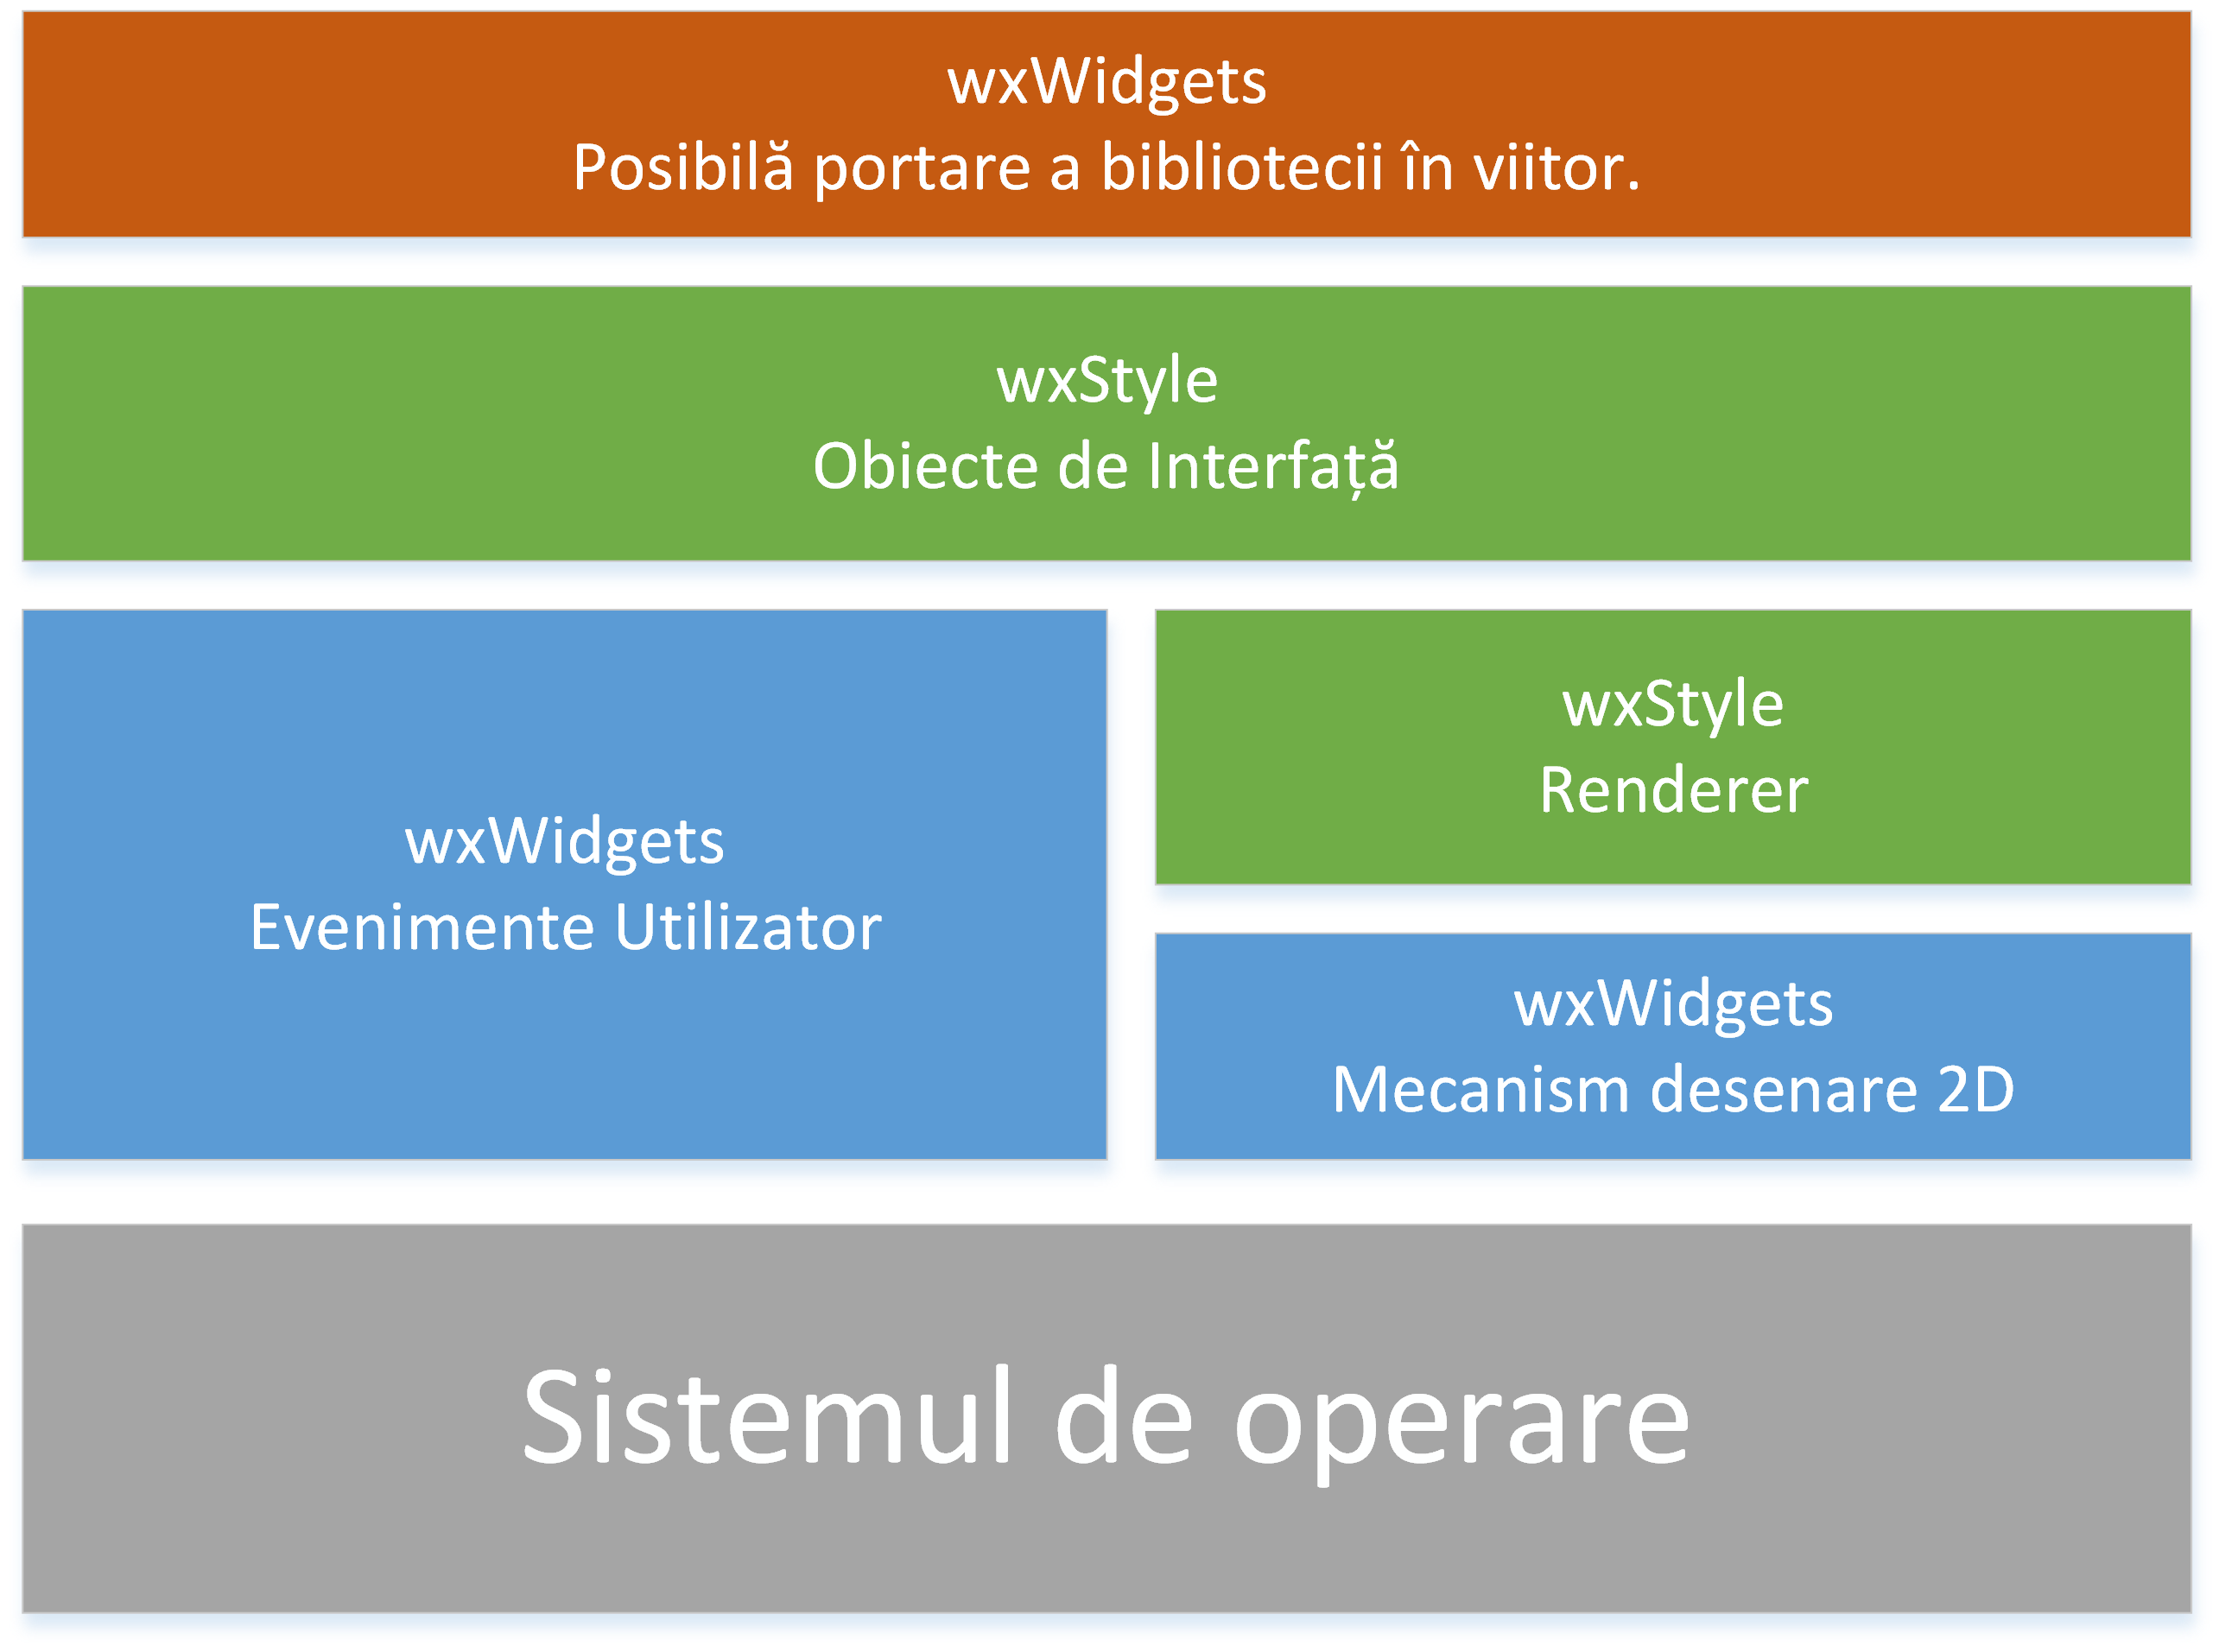
\includegraphics{img/ch2_arhitectura_bloc.png}
    \label{ch2_arhitectura_bloc}
    \caption{Arhitectura conceptual'a a bibliotecii wxStyle }
\end{figure}
\end{center}

\section{Mecanismului de stilizare}

Mecanismul de stilizare utilizeaz'a descrieri de stil pentru a specifica aspectele de prezentare ale unui obiect de interfa't'a. Un stil trebuie sa con'tin'a informatia necesar'a pentru:

\begin{enumerate}
\item Culorile de fundal si pentru text.
\item Font-ul utilizat la desenarea textului. 'In specifica'tia fontului includem: familia fontului, dimensiunea, greutatea fontului (sub'tire, normal sau bold) 'si 'inclina'tia fontului.
\item Umbra textului, care este descrisa printr-o deplasare relativ'a fa't'a de text 'si culoare.
\item Icoana utilizat'a op'tional de obiectul de interfa't'a va fi reprezentat'a prin numele imaginii.
\item Marginile interioare (numite si inset-uri), ce reprezint'a distan'ta dintre con'tinutul propriu-zis al unui obiect de interfa't'a 'si extremit'a'tile sale.
\item Aliniamentul textului at{\ia}t pe vertical'a c{\ia}t 'si pe orizontal'a.
\item Specificarea dac'a obiectul de interfa't'a este opac sau nu.
\item Un set de instruc'tiuni pentru desenarea fundalului.
\end{enumerate}

Urmatoarele reguli descriu modul de func'tionare al mecanismului de stilizare:

\begin{enumerate}
\item Toate obiectele de interfa't'a au ata'sate o procedur'a de desenare ce poate fi schimbat'a.
\item Toate obiectele de interfa't'a au ata'sat un stil complet, ce poate fi suprascris.
\item Defini'tiile de stil pot fi incomplete. Atunci c{\ia}nd unui obiect de interfa't'a i se ata'seaz'a un stil incomplet, con'tinutul acestuia va suprascrie doar acele tr'as'aturi care sunt definite.
\item Procedura de desenare ata'sat'a implicit unui obiect de interfa't'a utilizeaza stilul pentru a construi o reprezentare vizual'a.
\item Un fi'sier de stil con'tine mai multe stiluri ce pot fi ata'sate unei categorii de obiecte de interfa't'a (de exemplu tuturor butoanelor din aplica'tie).
\end{enumerate}

Setul de instruc'tiuni ata'sat unui stil descriu o primitiv'a de desenare 'impreuna cu parametrii acesteia. Este necesar'a posibilitatea desen'arii de imagini, forme 'si text cu dimensiuni 'si alinimente at{\ia}t relative c{\ia}t 'si absolute 'in cadrul unui obiect de interfa't'a.

\medskip

Componentele implementate 'in libr'aria wxStyle vor putea fi folosite 'impreun'a sau 'in locul celor implementate 'in cadrul libr'ariei wxWidgets. Un scop mai mare al acestei biblioteci, de'si imposibil de atins 'in cadrul lucr'arii de licent'a, este acela de a oferi o platform'a nou'a pentru wxWidgets, deasupra c'areia s'a poat'a fi portate toate obiectele de interfa't'a.